% Options for packages loaded elsewhere
\PassOptionsToPackage{unicode}{hyperref}
\PassOptionsToPackage{hyphens}{url}
%
\documentclass[
  12pt,
]{article}
\usepackage{lmodern}
\usepackage{amssymb,amsmath}
\usepackage{ifxetex,ifluatex}
\ifnum 0\ifxetex 1\fi\ifluatex 1\fi=0 % if pdftex
  \usepackage[T1]{fontenc}
  \usepackage[utf8]{inputenc}
  \usepackage{textcomp} % provide euro and other symbols
\else % if luatex or xetex
  \usepackage{unicode-math}
  \defaultfontfeatures{Scale=MatchLowercase}
  \defaultfontfeatures[\rmfamily]{Ligatures=TeX,Scale=1}
  \setmainfont[]{Times New Roman}
  \setsansfont[]{Quicksand}
\fi
% Use upquote if available, for straight quotes in verbatim environments
\IfFileExists{upquote.sty}{\usepackage{upquote}}{}
\IfFileExists{microtype.sty}{% use microtype if available
  \usepackage[]{microtype}
  \UseMicrotypeSet[protrusion]{basicmath} % disable protrusion for tt fonts
}{}
\makeatletter
\@ifundefined{KOMAClassName}{% if non-KOMA class
  \IfFileExists{parskip.sty}{%
    \usepackage{parskip}
  }{% else
    \setlength{\parindent}{0pt}
    \setlength{\parskip}{6pt plus 2pt minus 1pt}}
}{% if KOMA class
  \KOMAoptions{parskip=half}}
\makeatother
\usepackage{xcolor}
\IfFileExists{xurl.sty}{\usepackage{xurl}}{} % add URL line breaks if available
\IfFileExists{bookmark.sty}{\usepackage{bookmark}}{\usepackage{hyperref}}
\hypersetup{
  pdftitle={Register analysis of Chilean presidents speeches over 30 years},
  pdfauthor={Pamela Inostroza Fernández},
  hidelinks,
  pdfcreator={LaTeX via pandoc}}
\urlstyle{same} % disable monospaced font for URLs
\usepackage[margin=1in]{geometry}
\usepackage{longtable,booktabs}
% Correct order of tables after \paragraph or \subparagraph
\usepackage{etoolbox}
\makeatletter
\patchcmd\longtable{\par}{\if@noskipsec\mbox{}\fi\par}{}{}
\makeatother
% Allow footnotes in longtable head/foot
\IfFileExists{footnotehyper.sty}{\usepackage{footnotehyper}}{\usepackage{footnote}}
\makesavenoteenv{longtable}
\usepackage{graphicx,grffile}
\makeatletter
\def\maxwidth{\ifdim\Gin@nat@width>\linewidth\linewidth\else\Gin@nat@width\fi}
\def\maxheight{\ifdim\Gin@nat@height>\textheight\textheight\else\Gin@nat@height\fi}
\makeatother
% Scale images if necessary, so that they will not overflow the page
% margins by default, and it is still possible to overwrite the defaults
% using explicit options in \includegraphics[width, height, ...]{}
\setkeys{Gin}{width=\maxwidth,height=\maxheight,keepaspectratio}
% Set default figure placement to htbp
\makeatletter
\def\fps@figure{htbp}
\makeatother
\setlength{\emergencystretch}{3em} % prevent overfull lines
\providecommand{\tightlist}{%
  \setlength{\itemsep}{0pt}\setlength{\parskip}{0pt}}
\setcounter{secnumdepth}{5}
\usepackage[font=small,format=plain,labelfont=bf,up,textfont=normal,up,justification=justified,singlelinecheck=false]{caption} \usepackage{float} \usepackage{subfig}
\usepackage{booktabs}
\usepackage{longtable}
\usepackage{array}
\usepackage{multirow}
\usepackage{wrapfig}
\usepackage{float}
\usepackage{colortbl}
\usepackage{pdflscape}
\usepackage{tabu}
\usepackage{threeparttable}
\usepackage{threeparttablex}
\usepackage[normalem]{ulem}
\usepackage{makecell}
\usepackage{xcolor}

\title{Register analysis of Chilean presidents speeches over 30 years\thanks{All codes and txt files available \href{https://github.com/PamelaInostroza/MCL}{github.com/PamelaInostroza/MCL}. \textbf{Current version}: January 10, 2021; \textbf{Corresponding author}: \href{mailto:inostroza.f.pamela@gmail.com}{\nolinkurl{inostroza.f.pamela@gmail.com}}.}}
\author{Pamela Inostroza Fernández}
\date{Master in Statistics 2020/2021}

\begin{document}
\maketitle
\begin{abstract}
Factor analysis in addition to Correspondence Analysis was performed to identify characteristics of the last 31 speeches of Chilean presidents. The attributes of each speech, such as the number of words of different types, numbers, and the use of specific adverbs were used to identify how the structure of presidential speeches has changed accordingly with important events, like the change of the century, the first female president, the first right-wing president, and some catastrophes like 2010's earthquake and 2020's pandemic.
\end{abstract}

\newpage

\hypertarget{introduction}{%
\section{INTRODUCTION}\label{introduction}}

Every year, presidents had to communicate to the National Congress their main achievements and their legislative priorities for the near future. There is multiple information available for this type of texts. For this research, Chilean presidency transcripts will be used. The main objective will be to visualize some insights into the evolution of the linguistic used by each president according to the main events the country faced at the time.

Chilean speeches were chosen because they have a recent history that can help to identify some patterns in linguistic use. Data from the year 1990 when Chile got back to democracy from a dictatorship that took place for 17 years.

In the latest history of Chilean presidents, there have been 5 different presidents, 2 of them have repeated their mandate. In total 7 governments. This research will be focused in identify if the way of referencing to the congress/people in their speeches show specific characteristics.

Since the presidential function definitely has changed since the back of democracy it is expected that the speeches show this change and evolution of words and the way to address the main problems that the country faces at the time.

In this study it will be assumed that the president is the author of their speech (even though this is not literally), this research will not be focused in the team behind the writing of the speeches, this can lead to more in-depth research.

In order to identify the degree in which every group of speeches are different from one another, correspondence analysis will be performed. Here, many features will be obtained from each speech, some of these features are related to the length of the speech and frequencies of specific types of words. Also, it will include characteristics such as frequency of positive, negative words, bigrams, trigrams and other characteristics.

This research is performed completely on R software where libraries such as \emph{dplyr} for the management of the data, \emph{mclm} for specific functions for analysis of corpus linguistics, \emph{ca} to perform correspondence analysis, \emph{factanal} for exploratory factor analysis, \emph{knitr} to create a reproducible report, \emph{kableExtra} for tables visualization and \emph{ggplot}, \emph{ggwordcloud} and \emph{ggpubr} for plots visualizations.

\newpage

\hypertarget{description-of-dataset}{%
\section{DESCRIPTION OF DATASET}\label{description-of-dataset}}

The governmental speeches selected were produced in the same context from 1990 to 2020, 31 speeches in total. May 21th was established as the date when this public account speech should be performed every year. From the year 2017, this date was changed to June 1st\footnote{This date was changed exceptionally for the year 2020 regarding the global pandemic to July 31st}.

Each speech is available in plain text (.txt), this files can be downloaded from the site indicated previously, these files were read using \emph{get\_fnames} function from \textbf{mclm} package in R. For the use of Spanish language it is important to specify the encoding as ``UTF-8'', as the corpus contains the special character ``ñ'' and tildes in most vowels (such as á,é,í,ó,ú). From these files is this possible to extract all words used.

As a first approach to the data, a global cloud of words is performed, Figure \ref{fig:cloud} shows the most used words in all speeches studied, the size of the word in the graph indicates how many times the word was found in all sets of speeches. Words at the middle of the plot indicate the most used words, most visually identifiable words are ``Chile'', ``year'', ``country'', ``government'', ``law''.

\includegraphics{Figs/cloud-1.pdf}

\begin{table}[H]

\caption{\label{tab:cloud}Name and period of each president}
\begin{tabular}[t]{l|l|l}
\hline
N & Periodo & Name\\
\hline
1 & 1990-1993 & Patricio Aylwin\\
\hline
2 & 1994-1999 & Eduardo Frei\\
\hline
3 & 2000-2005 & Ricardo Lagos\\
\hline
4 & 2006-2009 & Michelle Bachelet\\
\hline
5 & 2010-2013 & Sebastian Pinera\\
\hline
6 & 2014-2017 & Michelle Bachelet\\
\hline
7 & 2018-2020 & Sebastian Pinera\\
\hline
\end{tabular}
\end{table}

The names read are saved for each year and president/mandate as a grouping variable identified by the option \emph{requested\_group = 1} from \emph{re\_retrieve\_first()} function, the table \ref{tab:cloud} indicate all the periods studied and the president in charge on those years.

It will be interesting to see how different attributes change over time, as an example, we can see in figure \ref{fig:descriptive1} the number of tokens and types found in each set of speeches. The longest speech was in 1997 and the shortest in 2001. The third period of Lagos as president shows the short amount of tokens compared to the rest of the speeches. In the plot also can be seen the most frequent type, for the first years of democracy, \emph{government} (gobierno) was most often used, then \emph{country} (país), the longest speech has \emph{development} (desarrollo) as the most frequent type. All following year use \emph{Chile} as principal type word, last 7 years \emph{country} is again the most common.

Much other information can be extracted from the corpus, as shown in figure \ref{fig:descriptive2}, the proportion of use of some attributes such as doubt adverbs, numbers, types and verbs is very different each year, and in some cases clear decrease/increase in their use.

This information is very interesting but not very helpful by itself in order to identify common patterns from every speech. For this reason, further analysis is needed, that allows us to combine all this information and obtain consolidate results about patterns in the speeches.

\begin{figure}
\centering
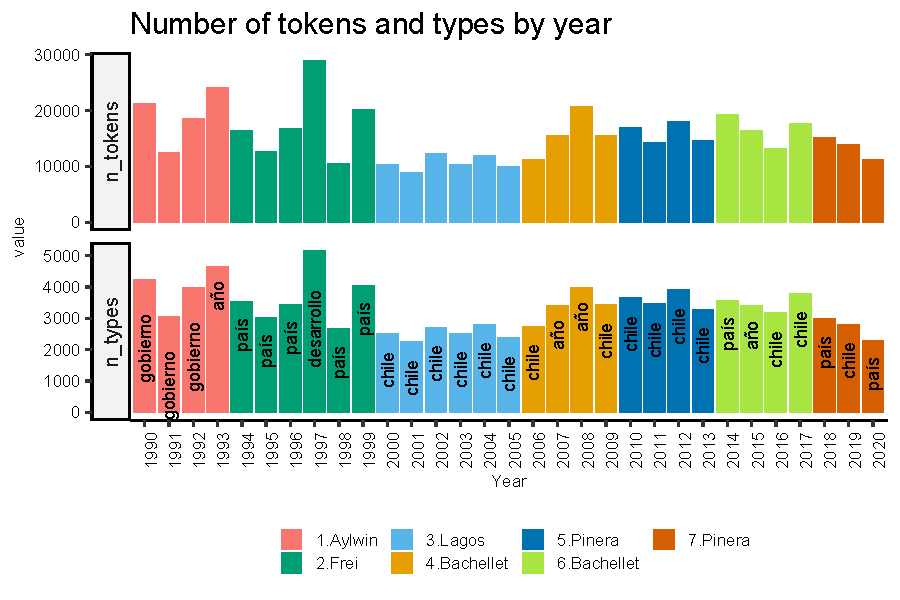
\includegraphics{Figs/descriptive1-1.pdf}
\caption{\label{fig:descriptive1}Number of tokens and types in speeches}
\end{figure}

\begin{figure}
\centering
\includegraphics{Figs/descriptive2-1.pdf}
\caption{\label{fig:descriptive2}Tendency (proportion of use) of speeches attributes}
\end{figure}

\newpage

\hypertarget{analysis}{%
\section{ANALYSIS}\label{analysis}}

The aim of this study is to review in which degree president speeches are related in the sense of similarities or dissimilarities. For this, many features will be extracted from the different corpus in order to obtain characterization that helps to perform this comparative analysis.

The attributes used to the reduction of dimension is listed as follows:

\begin{itemize}
\tightlist
\item
  word\_len: average word length (expressed as the number of characters)
\item
  p\_dig: the proportion of numbers used
\item
  p\_types: the proportion of types by total token \footnote{A graphical representation of most used types can be found in the annex, figure \ref{fig:correspondence1}}
\item
  p\_bigr: the proportion of bigrams used \footnote{A graphical representation of most used bigrams can be found in the annex, figure \ref{fig:correspondence2}}
\item
  p\_trigr: the proportion of trigrams used \footnote{A graphical representation of most used trigrams can be found in the annex, figure \ref{fig:correspondence3}}
\item
  p\_stopw: the proportion of stop words used
\item
  p\_funct: proportion of functional words
\item
  p\_verb: the proportion of verbs used
\item
  p\_mode: the proportion of modal adverbs \emph{(i.e., good, bad, simply, sincerely, fast)}
\item
  p\_advtim: the proportion of time adverbs \emph{(i.e., now, before, after, later, soon, yesterday, earlier, right now, yet, today)}
\item
  p\_advlug: the proportion of place adverbs \emph{(i.e., here, there, near, far, out, inside, around, aside, in, behind, front)}
\item
  p\_advqua: the proportion of quantity adverbs \emph{(i.e., much, a lot, very, almost, all, nothing, some, medium, more, less, also)}
\item
  p\_neg: the proportion of negative words \emph{(i.e., no, neither, never, ever, nobody, nothing, no one)}
\item
  p\_pos: the proportion of positive words \emph{(i.e., yes, too, some, always)}
\item
  p\_dou: the proportion of doubt adverbs \emph{(i.e., might, maybe, perhaps)}
\end{itemize}

\hypertarget{correspondence-analysis}{%
\subsection{Correspondence analysis}\label{correspondence-analysis}}

Correspondence analysis is a dimension reduction technique that allows us to create relations among rows, columns and between rows and columns. This type of analysis is very flexible in the sense that no extra restrictions are imposed on contingency tables.

The main idea resides in a dimensional reduction, where each observation is represented by a point and each attribute as a dimension. This representation can be visualized in a two-dimensional space where a cloud of points indicates the relation between new dimensions.

\begin{table}[H]

\caption{\label{tab:corrtb}Variance explained by each dimension}
\begin{tabular}[t]{l|r|r|r}
\hline
  & Eigenvalue & Variance explained & Cumulative 
Variance explained\\
\hline
Dim.1 & 0.022 & 49.2 & 49.2\\
\hline
Dim.2 & 0.011 & 23.4 & 72.6\\
\hline
Dim.3 & 0.007 & 15.7 & 88.3\\
\hline
Dim.4 & 0.003 & 7.3 & 95.6\\
\hline
\end{tabular}
\end{table}

As indicated in table \ref{tab:corrtb}, 72.6\% of the total variance can be explained by reducing all the attributes in 2 dimensions, figure \ref{fig:corresp} shows how these 2 dimensions are distributed. It can be seen that most of the attributes are together in the II quadrant (upper left), from here we can say that is possible to reduce the dimensions even more in order to facilitate the interpretation. For this reason, factor analysis is also performed in order to reduce the number of attributes (15) into a few factors (4) that summarize all similar attributes.

\begin{figure}
\centering
\includegraphics{Figs/corresp-1.pdf}
\caption{\label{fig:corresp}Correspondence analysis of attributes}
\end{figure}

\hypertarget{factor-analysis}{%
\subsection{Factor analysis}\label{factor-analysis}}

After performing factor analysis, it is possible to indicate that attributes such as the proportion of stop and functional words, time, quantity and modal adverbs, negative words are strongly related, hence, it is possible to combine them and obtain a new factor. It is important to mention that when the loading is negative, as for modal adverbs and length of words, this means that the attribute should be read inversely. This factor could be named as \textbf{Single words, short length}. As Factor 2, can be combined attributes related to the proportion of types, bigrams and trigrams, named as \textbf{Composed sentences}. Factor 3 is mainly composed by the proportion of verbs and digits, it was called, \textbf{Use of verbs and no numbers}. Lastly, factor 4 include doubt adverbs, it was called \textbf{Use of hesitant words}. With this reduction of attributes, that explain more than 80\% of the total variance, it is possible to redo the previous graph where the relations between the attributes and each year can be clearly differentiated by this four interpretable factors.

\begin{table}[H]

\caption{\label{tab:factor}Factors identified}
\fontsize{10}{12}\selectfont
\begin{tabu} to \linewidth {>{\raggedright}X>{\raggedleft}X>{\raggedleft}X>{\raggedleft}X>{\raggedleft}X}
\hline
Attribute & F1-Use of single words, short lenght & F2-Use of composed sentences & F4-Use of verbs but less numbers & F5-Use of hesitant adverbs\\
\hline
p\_funct & 0.880 &  &  & \\
\hline
p\_stopw & 0.867 &  &  & \\
\hline
p\_advtim & 0.690 &  &  & \\
\hline
p\_advqua & 0.658 &  &  & -0.589\\
\hline
p\_neg & 0.536 &  &  & \\
\hline
p\_mode & -0.618 &  &  & \\
\hline
word\_len & -0.960 &  &  & \\
\hline
p\_bigr &  & 0.980 &  & \\
\hline
p\_types &  & 0.946 &  & \\
\hline
p\_trigr &  & 0.941 &  & \\
\hline
p\_verb &  &  & 0.702 & \\
\hline
p\_dig &  &  & -0.875 & \\
\hline
p\_advdou &  &  &  & 0.756\\
\hline
\end{tabu}
\end{table}

With this graphical visualisation it is possible to identify that first two periods and social democrats presidents, figures \ref{fig:plot-1} and \ref{fig:plot-2} \emph{(1.Aylwin, 2.Frei)}, in F1-F2 biplot are concentrated in the left side of the plot, which corresponds to longer speeches and use of single words. Similar behaviour for both periods is found in F3-F4 biplot, in both cases, their speeches are concentrated in the upper side, which means more use of doubt adverbs.

During the third period, figure \ref{fig:plot-3} \emph{(3.Lagos)}, the first socialist president after return to the democracy, another distribution can be seen in the graphs compared to the previous ones, as in the first biplot F1-F2, speeches are concentrated in the upper right quadrant which means shorter than other speeches but use more single words, types, bigrams and trigrams. In the second plot, speeches are mainly in the upper left quadrant, this means that the use of doubt adverbs was common as previous presidents but after the year 2000 the use of verbs decreased and the use of numbers increased.

\begin{figure}[H]
\subfloat[Biplot 1.Aylwin\label{fig:plot-1}]{\includegraphics{Figs/plot-1} }\newline\subfloat[Biplot 2.Frei\label{fig:plot-2}]{\includegraphics{Figs/plot-2} }\newline\subfloat[Biplot 3.Lagos\label{fig:plot-3}]{\includegraphics{Figs/plot-3} }\newline\subfloat[Biplot 4.Bachellet\label{fig:plot-4}]{\includegraphics{Figs/plot-4} }\newline
\end{figure}

\begin{figure}[H]
\subfloat[Biplot 5.Pinera\label{fig:plot-5}]{\includegraphics{Figs/plot-5} }\newline\subfloat[Biplot 6.Bachellet\label{fig:plot-6}]{\includegraphics{Figs/plot-6} }\newline\subfloat[Biplot 7.Pinera\label{fig:plot-7}]{\includegraphics{Figs/plot-7} }\caption{Correspondence analysis of 4 main factors}\label{fig:plot}
\end{figure}

Continuing the tendency from the previous period, in figure \ref{fig:plot-4}, fourth period endorsed by the second socialist and first female president \emph{(4.Bachellet)}, her speeches are concentrated in the upper right quadrant, maintaining shorter speeches with use of single words and more types and bigrams/trigrams with exception of the year 2008, where fewer types/bigrams/trigrams where used. For the second F3-F4 biplot, the tendency changed dramatically as these speeches are mainly concentrated in the first quadrant, which means that fewer doubt adverbs were used, and more verbs and fewer digits.

In the fifth period \emph{(5.Pinera)}, the first right-wing president since the back to the democracy, from national renovation party. In figure \ref{fig:plot-5} the distribution of his speeches are almost right in the middle in F1-F2 biplot, this means that the length of the speeches is medium compared to the other speeches, and also in the use of single terms and composed types, bigrams and trigrams. In the second biplot (F3-F4), can be seen that no doubt adverbs are used compared to the other speeches, fewer verbs and more numbers are used after the first year of his mandate 2010 when the country suffered a massive earthquake.

For the second period of \emph{(6.Bachellet)}, figure \ref{fig:plot-6} shows that even though the position in the middle of the plot is maintained as in her first period (F1-F2 biplot), this time is more disperse (in 2014 less use of composed words and in year 2016, more use of composed words). For the second biplot F3-F4, even though the use of doubt adverbs is lower, after the first year, more numbers are used and fewer verbs compared to other speeches.

Finally, the last period studied \emph{(7.Pinera)}, and the second period for the only right-wing president, figure \ref{fig:plot-7} shows the shortest speeches of all in F1-F2 biplot, with more use of single words, and less use of types, bigrams/trigrams. In the second biplot F3-F4, the tendency of no use of doubt adverbs was broken on the year 2020 when the COVID-19 pandemic occurs and more verb is used and fewer numbers in the three years.

\hypertarget{conclusion}{%
\section{CONCLUSION}\label{conclusion}}

Visually, it is easy to identify the main differences between characteristics of the speeches of each president, and thanks to the reduction of dimension it is easier to interpret.

As a conclusion, without going into any deep political analysis, the attributes selected from each speech, allow us to identify the main behaviour of the way the speeches were performed based on the period they were given.

It is clear the caution that is used in the wording until the year 2000 (first 10 years of democracy), maybe this change was because of the century change and the new technological development starting to be more accessible.

Another important event can be seen when the first woman president was elected, even though the previous president was from the same party, no relation can be found in the characteristic of their speeches.

The most obvious change can be seen when the first right-wing president was in charge, sadly the very first year he started, a massive earthquake (8.8Mww) occur in Chile and this can be seen in the analysis too.

Finally, the last period, the lowest approval rating president show a completely different characterization of his speeches, even different from his previous mandate. Also, the cautious wording is evidenced for the year 2020 when the pandemic occurs.

\end{document}
